\documentclass[a5paper,leqno,fontsize=10pt]{book}
\usepackage{tcolorbox}
\definecolor{headercolor}{HTML}{F5F5F5}
\definecolor{headercolor}{HTML}{E9EFEF}
\usepackage[margin=0.53in]{geometry}
\usepackage{fancyhdr,tikz,tkz-tab,picins,multicol}
\usetikzlibrary[calc,intersections,through,backgrounds]
 \usepackage{fancyhdr,wrapfig,amsmath,tcolorbox}
 \renewcommand{\baselinestretch}{1.7}
 \usepackage{tkz-euclide,tikz,tikz-3dplot}
  \usetikzlibrary{angles,quotes}
 \newcommand{\so}{\textcolor{blue}{\bfseries{ដំណោះស្រាយ}}}
 \usepgflibrary{arrows.meta}
 \usetkzobj{all} 
\makeindex
\usepackage{mdframed} 
\usepackage{xwatermark,arcs}
\usetikzlibrary{shadings} 
\usetikzlibrary{decorations.pathmorphing}
\tcbset{colback=green!10!white}
\usepackage{amsthm}
\tcolorboxenvironment{proof}{blanker,breakable,left=5mm,
	before skip=10pt,after skip=10pt,borderline west={1mm}{0pt}{red!10!cyan}}
\def\theoremname{ទ្រឹស្ដីបទ}
\def\corollaryname{វិបាក}
\def\hint{\noindent\bfseries \textcolor{blue}{\underline{ការណែនាំ}}}
\def\propositionname{លក្ខណៈ}
\def\definitionname{និយមន័យ}
\def\examplename{ឧទាហរណ៍}
\def\exercisename{លំហាត់}
\def\tableofcontentsename{មាតិកា}
\def\answername{ចម្លើយ}
\def\remarkname{សម្គាល់}
\def\generalname{លក្ខណៈ}
\def\hinname{\bfseries ណែនាំ\quad}
\def\practicename{ប្រតិបត្តិ}
\def\formulaname{រូបមន្ត}
\usepackage{fancyhdr}
\usepackage{newbook1}
\pagestyle{fancy}
\XeTeXlinebreaklocale "khm" % allow line breaks 
\XeTeXlinebreakskip = 0pt plus 1pt minus 1pt
\renewcommand\headrulewidth{1pt}
\renewcommand\footrulewidth{0pt}
%\rfoot{}
\cfoot{\thepage}
\makeatletter
\patchcmd{\over@under@arc}
{\@gobbletwo}{\@gobblethree}{}{}
\begin{document}
\chapter{គន្លឹះធរណីមាត្រសំខាន់ៗ}
\subsection*{ការបង្ហាញប្រភេទត្រីកោណ}
\begin{enumerate}
	\item {{\color{blue}\bfseries ត្រីកោណសមបាត}}
	\begin{itemize}
		\begin{minipage}{0.56\linewidth}
			\item $ \triangle ABC $ មាន : \quad $ [AB]\cong [AC]$ \\  $\Longrightarrow $ \quad  \fbox{~$ \triangle ABC$~ សមបាតកំពូល $ A $~}
			\item $ \triangle ABC $ មាន : \quad $ \angle B\cong\angle C$ \\
			$\Longrightarrow$ \quad \fbox{ ~$  \triangle ABC$~ សមបាតកំពូល $ A $~}\\
		\end{minipage}
		\begin{minipage}{0.54\linewidth}
			\begin{tikzpicture}[scale=0.8]
			\tkzDefPoint(0,0){B}
			\tkzDefPoint(3,0){C}
			\tkzDefPoint(1.5,2){A}
			\tkzMarkSegments[size=0.8 mm,mark=|](A,B A,C)
			\tkzLabelPoints[below left](B)
			\tkzLabelPoints[below right](C)
			\tkzLabelPoints[above](A)
			\tkzMarkAngles[size=0.4,fill=green!30](C,B,A A,C,B)
			\tkzDrawSegments[color=cyan](A,B B,C C,A)​
			\tkzMarkAngles[size=0.4](C,B,A A,C,B)
			\tkzMarkAngles[size=0.45](C,B,A A,C,B)
			\tkzDrawPoints(A,B,C)
			\end{tikzpicture}
		\end{minipage} 
		\item 	$ \triangle ABC $ មាន :\\[-5pt]
		\begin{minipage}{0.59\linewidth}
			$ \begin{aligned}[t]
			\text{កំពស់}~[AH]~~&\text{ជាកន្លះបន្ទាត់ពុះនៃ មុំ}~\angle A\\[-3pt]
			~&\text{ឬ~~ជាមេដ្យាន}~\angle A\\[-3pt]
			&\text{ឬ~~ជាមេដ្យាទ័រនៃបាត}~[BC]\\[-3pt]
			&\text{ឬ~~ជាអ័ក្សបំលែងឆ្លុះ}
			\end{aligned} $
		\end{minipage}
		\begin{minipage}{0.35\linewidth}
			\begin{tikzpicture}[scale=0.8]
			\tkzInit[xmin=-0.2,xmax=4.2,ymin=-0.4,ymax=3]
			\tkzClip[space=.5] 
			\tkzDefPoint(0,0){B}
			\tkzDefPoint(3,0){C}
			\tkzDefPoint(1.5,2){A}
			\tkzMarkSegments[size=0.8 mm,mark=|](A,B A,C)
			\tkzLabelPoints[below left](B)
			\tkzLabelPoints[below right](C)
			\tkzLabelPoints[above](A)
			\tkzDefPointBy[projection=onto B--C](A)\tkzGetPoint{H}
			\tkzMarkRightAngles(A,H,C)
			\tkzDrawSegments[color=cyan](A,B B,C C,A A,H)​
			\tkzDrawPoint(H)\tkzLabelPoints[below](H)
			\tkzDrawPoints(A,B,C)	
			\end{tikzpicture}
		\end{minipage}\\[-5pt]
		$ \Longrightarrow$ \fbox{ $~~\triangle ABC $ ជាត្រីកោណសមបាត~}
	\end{itemize}
	\item {\color{blue}\bfseries ត្រីកោណកែងសមបាត }\\
	\begin{minipage}{0.69\linewidth}
		ត្រូវបង្ហាញថា $ \triangle ABC $ សមបាតជាមុនសិន \\
		ហើយ $ \triangle ABC $~សមបាតកំពូល $ A $​ មាន :~~
		$ \hat{A}=90^\circ $\\
		$ \Longrightarrow $~~\fbox{~$ \triangle ABC $ ~ជាត្រីកោណកែងសមបាតកំពូល $ A $}
	\end{minipage}
	\begin{minipage}{0.35\linewidth}
		\begin{tikzpicture}[scale=0.9]
		\tkzInit[xmin=0,xmax=1.5,ymin=0,ymax=1.5]
		\tkzClip[space=.5] 
		\tkzDefPoint(0,0){A}
		\tkzDefPoint(1.5,0){C}
		\tkzDefPoint(0,1.5){B}
		\tkzMarkRightAngles(B,A,C)
		\tkzDrawSegments[color=cyan](A,C C,B A,B)​
		\tkzMarkSegments[size=0.8 mm,mark=|](A,B A,C)
		\tkzDrawPoint(A)\tkzLabelPoints[below](A)	
		\tkzDrawPoints(A,C,B)
		\tkzLabelPoints[below right](C)
		\tkzLabelPoints[above](B)
		\end{tikzpicture}
	\end{minipage}
	\item {{\color{blue}\bfseries ត្រីកោណសម័ង្ស}}\\
	បើឃើញ  $ \triangle ABC $ មានៈ
	\begin{itemize}
		\begin{minipage}{0.67\linewidth}
			\item$ [AB]\cong [BC]\cong [AC] $\\[4pt]
			$ \Longrightarrow$ \fbox{~ $ \triangle ABC $ ជាត្រីកោណសម័ង្ស~}
			\item $ \triangle ABC $ មានៈ\quad
			$ \widehat{A}=\widehat{B}=\widehat{C} $\\
			$ \Longrightarrow~$ \fbox{~ $\triangle ABC $ ជាត្រីកោណសម័ង្ស~}
		\end{minipage}
		\begin{minipage}{0.4\linewidth}
			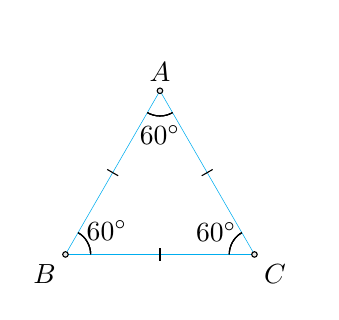
\begin{tikzpicture}[scale=0.8]
			\tkzInit[xmin=-0.1,xmax=3.4,ymin=-0.1,ymax=3.1]
			\tkzClip[space=.5] 
			\tkzDefPoint(0,0){B}
			\tkzDefShiftPoint[B](0:3){C}
			\tkzDefShiftPoint[B](60:3){A}
			\tkzMarkAngles[size=0.4,fill=green!30](C,B,A A,C,B B,A,C)
			\tkzDrawSegments[color=cyan](A,B B,C C,A)
			\tkzMarkSegments[size=0.8 mm,mark=|](A,B A,C C,B)
			\tkzDrawPoints(A,B,C)
			\tkzLabelPoints[below left](B)
			\tkzLabelPoints[below right](C)
			\tkzLabelPoints[above](A)
			\tkzMarkAngles[size=0.4](C,B,A A,C,B B,A,C)
			\tkzMarkAngles[size=0.4](C,B,A A,C,B B,A,C)
			\tkzLabelAngles[pos=0.76](C,B,A){$ 60^\circ $}
			\tkzLabelAngles[pos=0.7](A,C,B){$ 60^\circ $}
			\tkzLabelAngles[pos=0.7](B,A,C){$ 60^\circ $}
			\end{tikzpicture}
		\end{minipage}
		\newpage
		\item $ \triangle ABC $ សមបាត​ មានមុំុំ ១ ស្មើ ~~  $ 60^\circ $\\[5pt]
		$ \Longrightarrow $~~\fbox{$ \triangle ABC $ ​ ជាត្រីកោណសម័ង្ស}
	\end{itemize}	
	\item {\color{blue}\bfseries ត្រីកោណកែង}
	\begin{itemize}
		\begin{minipage}{0.58\linewidth}
			\item បើឃើញ  $ \triangle ABC $ មាន $ \widehat{A} =90^\circ $\\
			$ \Longrightarrow $~$ ABC $ ជាត្រីកោណកែងត្រង់ $ A $ 
			\item មុំចារឹកកន្លះរង្វង់ជាមុំកែង
		\end{minipage}
		\begin{minipage}{0.44\linewidth}
			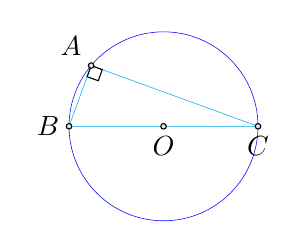
\begin{tikzpicture}[scale=0.6]
			\tkzDefPoint(0,0){B}
			\tkzDefPoint(4,0){C}
			\tkzDefMidPoint(B,C)\tkzGetPoint{O}
			\tkzDrawCircle[color=blue](O,B)
			\tkzDefPointBy[rotation=center O angle -40 ](B)
			\tkzGetPoint{A}
			\tkzDrawPolygon[color=cyan](A,B,C)
			\tkzLabelPoints(C,O)
			\tkzLabelPoints[above left](A)
			\tkzLabelPoints[left](B)
			\tkzMarkRightAngle(B,A,C)
			\tkzDrawPoints(B,C,O,A)
			\end{tikzpicture}
		\end{minipage}
		\begin{minipage}{0.6\linewidth}
			\item $ \triangle ABC $ មានៈ\\
			$ [AM] $ ជាមេដ្យាន \\
			$ [AM]=\dfrac{[BC]}{2} $\\
			$ \Longrightarrow~$ $ \triangle ABC $ កែងត្រង់ $ A $
		\end{minipage}
		\begin{minipage}{0.41\linewidth}
			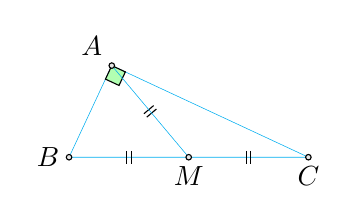
\begin{tikzpicture}[scale=0.76]
			\tkzDefPoint(0,0){B}
			\tkzDefPoint(4,0){C}
			\tkzDefMidPoint(B,C)\tkzGetPoint{M}
			\tkzDefPointBy[rotation=center M angle -50 ](B)
			\tkzGetPoint{A}
			\tkzDrawPolygon[color=cyan](A,B,C)
			\tkzLabelPoints(C,M)
			\tkzLabelPoints[above left](A)
			\tkzLabelPoints[left](B)
			\tkzMarkSegments[size=0.8 mm,mark=||](A,M B,M M,C)
			\tkzMarkRightAngle[fill=green!30](B,A,C)
			\tkzDrawSegment[color=cyan](A,M)
			\tkzDrawPoints(B,C,M,A)
			\end{tikzpicture}
		\end{minipage}
	\end{itemize}
	\item  {\color{blue}\bfseries ត្រីកោណកន្លះសម័ង្ស}\\
	\begin{itemize}
		\begin{minipage}{0.6\linewidth}
			\item $ \triangle ABC $ កែងត្រង់ ~$ A $\\
			ហើយមាន $ \widehat{B}=30^\circ ~ $( ឬ  $ \widehat{C}=60^\circ $)\\[5pt]
			$ \Longrightarrow~$ \fbox{~ $\triangle ABC $~ជាត្រីកោណកន្លះសម័ង្ស~}\\
			\item ត្រីកោណកែង~ $ ABC $~ មានៈ\quad  $|AC|=\dfrac{|BC|}{2}$\\[5pt]
			$ \Longrightarrow $~\fbox{~$ \triangle ABC $ ជាត្រីកោណកន្លះសម័ង្ស~}
		\end{minipage}
		\begin{minipage}{0.43\linewidth}
			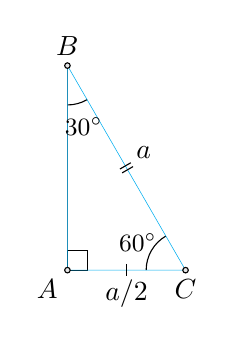
\begin{tikzpicture} 
			\tkzDefPoint(0,0){O}	
			\tkzDefShiftPoint[O](0:3){C}
			\tkzDefShiftPoint[C](120:3){B}
			\tkzDefMidPoint(O,C)\tkzGetPoint{A}
			\tkzDrawSegment(A,B)
			\tkzLabelPoints(C)
			\tkzMarkRightAngles(B,A,C)
			\tkzMarkAngles[size=0.5,fill=green!30](B,C,A  A,B,C)
			\tkzDrawPolygon[color=cyan](A,B,C)
			\tkzLabelAngles[pos=0.8](A,B,C){\small $ 30^\circ $}
			\tkzLabelAngles[pos=0.7](B,C,A){\small $ 60^\circ $}
			\tkzDrawPoints(A,B,C)
			\tkzLabelPoints[below left](A)  
			\tkzLabelPoints[above](B)
			\tkzMarkSegments[size=0.8 mm,mark=||](B,C)
			\tkzMarkSegments[size=0.8 mm,mark=|](A,C)
			\tkzLabelSegment[below](A,C){ $ a/2 $}
			\tkzLabelSegment[above right](B,C){  $a $}
			\end{tikzpicture}
		\end{minipage}
	\end{itemize}
\end{enumerate}
\subsection*{បន្ទាត់ពីរស្របគ្នា}
\begin{enumerate}
	\item {\color{blue}\bfseries បន្ទាត់២​ស្របនឹងបន្ទាត់តែមួយ}\\
	\begin{minipage}{0.66\linewidth}
		បើឃើញ\quad $ \begin{aligned}
		(d)\parallel (\Delta)\\[-0.6pt]
		(d')\parallel (\Delta)
		\end{aligned}\Longrightarrow~$~ \fbox{~~$ (d)\parallel (d')$~~} \\
	\end{minipage}
	\begin{minipage}{0.5\linewidth}
		\begin{tikzpicture}
		\tkzDefPoint(0,0){A}
		\tkzDefPoint(2,0){B}
		\tkzDefPoint(0,0.6){C}
		\tkzDefPoint(2,0.6){D}
		\tkzDefPoint(0,-0.6){E}
		\tkzDefPoint(2,-0.6){F}
		\tkzDrawLine[color=cyan,end=$ (d) $](A,B)
		\tkzDrawLine[color=cyan,end=$ (d') $](C,D)
		\tkzDrawLine[color=cyan,end=$ (\Delta) $](E,F)
		\end{tikzpicture}
	\end{minipage}
	\item {\color{blue}\bfseries បន្ទាត់២​កែងនឹងបន្ទាត់តែមួយ}\\
	បើឃើញ\quad $ \begin{aligned}
	(d)\perp (\Delta)\\
	(d')\perp (\Delta)
	\end{aligned}$
	$ \Longrightarrow~~$ \fbox{~~$ (d)\parallel (d')$~~}\qquad\qquad\quad
	\begin{minipage}{0.5\linewidth}
		\begin{tikzpicture}
		\tkzDefPoint(0,0){A}
		\tkzDefPoint(2,0){B}
		\tkzDefPoint(0,0.6){C}
		\tkzDefPoint(2,0.6){D}
		\tkzDefPoint(1.5,1){E}
		\tkzDefPoint(1.5,-0.3){F}
		\tkzInterLL(A,B)(E,F)\tkzGetPoint{H}
		\tkzInterLL(C,D)(E,F)\tkzGetPoint{K}
		\tkzMarkRightAngles[fill=magenta!20](A,H,E C,K,E)
		\tkzDrawLine[color=cyan,end=$ (d) $](A,B)
		\tkzDrawLine[color=cyan,end=$ (d') $](C,D)
		\tkzDrawLine[end=$ (\Delta) $](F,E)
		\end{tikzpicture}
	\end{minipage}
	\item {\color{blue}\bfseries មុំនៃបន្ទាត់ $ (d)\parallel (d') $ និងខ្នាត់ $ (\Delta) $}\\
	\begin{minipage}{0.56\linewidth}
		$\begin{aligned}[t]
		\text{បើឃើញ~~ }\widehat{A_1}&=\widehat{B_1} ~~\Longrightarrow~~
		(d)\parallel (d')~\\
		(~\text{ឬ}~ \widehat{A_3}&=\widehat{B_1})\quad \text{(~មុំឆ្លាស់ក្នុង~)}\\
		(~\text{ឬ}~~\widehat{A_2}+\widehat{B_1}&=180^\circ)\quad \text{(មុំរួមខាង)}
		\end{aligned}$ 
	\end{minipage}
	\begin{minipage}{0.4\linewidth}
		\begin{tikzpicture}[scale=0.72]
		\tkzDefPoint(0,0){A}
		\tkzDefPoint(4,0){B}
		\tkzDefPoint(0,-2){C}
		\tkzDefPoint(1,-2.2){x}
		\tkzDefLine[parallel=through C](A,B)\tkzGetPoint{D}
		\tkzDefPoint(2.5,0.4){y}
		\tkzDrawLines[color=cyan,end=$ (d_1) $](C,D)
		\tkzDrawLines[color=cyan,end=$ (d_2) $](A,B)
		\tkzDrawLine(x,y)
		\tkzInterLL(A,B)(x,y)\tkzGetPoint{H}
		\tkzInterLL(C,D)(x,y)\tkzGetPoint{K}
		\tkzMarkAngles[size=0.47](A,H,x  D,K,y)
		\tkzMarkAngles[size=0.5](A,H,x  D,K,y)
		\tkzLabelAngles[pos=0.5](x,H,A){$ 1 $}
		\tkzLabelAngle[pos=0.5](y,H,A){$ A $}
		\tkzLabelAngles[pos=0.5](x,H,B){$ 2 $}
		\tkzLabelAngles[pos=0.7 5](y,K,D){$ 1 $}
		\tkzLabelAngle[pos=0.5](y,K,C){$ B$}
		\tkzText(1.55,-0.4){$ 3 $}
		\tkzText(0.6,-2.3){$ 3$}
		\tkzLabelAngles[pos=0.5](x,K,B){$ 2 $}
		\tkzDrawPoints(H,K)
		\end{tikzpicture}	
	\end{minipage}
	\item {\color{blue}\bfseries បន្ទាត់ភ្ជាប់ចំនុចកណ្តាលជ្រុង២របស់ត្រីកោណ}\\
	\begin{minipage}{0.63\linewidth}
		បើដឹងថា  ក្នុងត្រីកោណ $ ABC $ មាន\\
		$ 	\begin{aligned}
		M ~ \text{កណ្តាល}~  [AC] \\
		N  ~ \text{កណ្តាល}~  [AB] 	
		\end{aligned}\quad\Longrightarrow~(MN)\parallel (BC) $
	\end{minipage}
	\begin{minipage}{0.5\linewidth}
		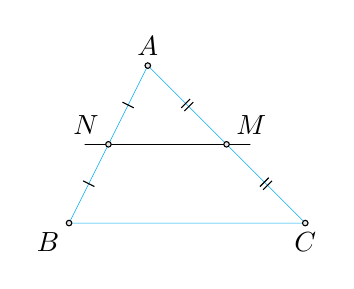
\begin{tikzpicture}
		\tkzDefPoint(0,0){B}
		\tkzDefPoint(3,0){C}
		\tkzDefPoint(1,2){A}
		\tkzDefBarycentricPoint(A=1,C=1)
		\tkzGetPoint{M}
		\tkzDefLine[parallel=through M](B,C)\tkzGetPoint{I}
		\tkzInterLL(A,B)(M,I)\tkzGetPoint{N}
		\tkzDrawPolygon[color=cyan](A,B,C)
		\tkzDrawSegments(M,N)
		\tkzLabelPoints(C)
		\tkzDrawLine(M,N)
		\tkzMarkSegments[size=0.8 mm,mark=|](B,N N,A)
		\tkzMarkSegments[size=0.8 mm,mark=||](C,M M,A)
		\tkzLabelPoints[above](A)
		\tkzLabelPoints[above right](M)
		\tkzLabelPoints[above left](N)
		\tkzDrawPoints(A,B,C,M,N)
		\tkzLabelPoints[below left](B)
		\end{tikzpicture}
	\end{minipage}
	\item {\color{blue}\bfseries បាតមធ្យមរបស់ត្រីកោណ ឬ ចតុកោណព្នាយ}\\
	\begin{minipage}{0.6\linewidth}
		\begin{itemize}
			\item បើដឹងថា ក្នុង $ \triangle ABC $ មានៈ\\
			$ [MN] $ បាតមធ្យម  \\
			$ \Longrightarrow~(MN)\parallel (BC)~,~|MN|=\dfrac{|BC|}{2} $
		\end{itemize}
	\end{minipage}
	\begin{minipage}{0.45\linewidth}
		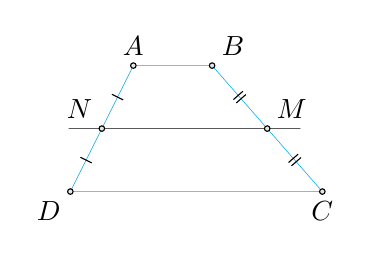
\begin{tikzpicture}[scale=0.8]
		\tkzDefPoint(0,0){D}
		\tkzDefPoint(4,0){C}
		\tkzDefPoint(1,2){A}
		\tkzDefPoint(2.25,2){B}
		\tkzDefBarycentricPoint(B=1,C=1)
		\tkzGetPoint{M}
		\tkzDefLine[parallel=through M](D,C)\tkzGetPoint{I}
		\tkzInterLL(A,D)(M,I)\tkzGetPoint{N}
		\tkzDrawPolygon[color=cyan](A,B,C,D)
		\tkzDrawLine(M,N)
		\tkzDrawPoints(A,B,C,D,M,N)
		\tkzLabelPoints(C)	
		\tkzMarkSegments[size=0.8 mm,mark=|](D,N N,A)
		\tkzMarkSegments[size=0.8 mm,mark=||](B,M M,C)
		\tkzLabelPoints[above](A)
		\tkzLabelPoints[above right](M)
		\tkzLabelPoints[above left](N)
		\tkzLabelPoints[above right](B)
		\tkzLabelPoints[below left](D)
		\end{tikzpicture}
	\end{minipage}
	\begin{itemize}
		\item ក្នុងចតុកោណព្នាយ $ ABCD $ មានៈ\\
		$ [MN] $ បាតមធ្យម 
		$ \Longrightarrow \begin{cases}
		[MN]\parallel[AB]\parallel [CD]\\
		|NM|=\dfrac{|AB|+|CD|}{2}
		\end{cases} $
	\end{itemize}
	\item {\color{blue}\bfseries ជ្រុងឈមនៃប្រលេឡូក្រាម ឬ (ប្រលេឡូក្រាមពិសេស)}\\
	\begin{minipage}{0.69\linewidth}
		បើដឹងថាៈ\quad $ ABCD $ ជាប្រលេឡូក្រាម\\
		(ឬ ចតុកោណស្មើ ឬ​ ការេ)\\
		$ \Longrightarrow~ $~ ~~$ [AB]~\parallel ~[CD] $
	\end{minipage}
	\begin{minipage}{0.45\linewidth}
		\begin{tikzpicture}[scale=0.7]
		\tkzDefPoints{0/0/D,2/0/C,2/2/B,0/2/A}
		\tkzDrawSegments[color=cyan](D,A A,B B,C C,D)
		\tkzLabelPoints[above left](A)
		\tkzLabelPoints[above right](B)
		\tkzLabelPoints[below right](C)
		\tkzLabelPoints[below left](D)
		\tkzDrawPoints(A,B,C,D)
		\end{tikzpicture}
	\end{minipage}
	\item {\color{blue}\bfseries ធ្នូប៉ុនគ្នាក្នុងរង្វង់}\\
	\begin{minipage}{0.65\linewidth}
		ក្នុងរង្វង់ $ (S) $ បើគេដឹងថាៈ ~\\
		$ \smile AB~\cong~ \smile~ CD$~
		$ \Longrightarrow~~ [AC]~\parallel ~[BD] $
	\end{minipage}
	\begin{minipage}{0.4\linewidth}
		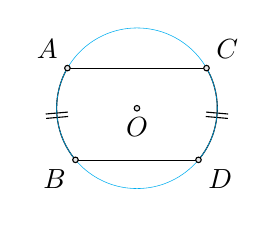
\begin{tikzpicture}[scale=0.68]
		\tkzDefPoint(-1.5,0){P}
		\tkzDefPoint(0,0){O}
		\tkzDefPoint(1.5,0){Q}
		\tkzDefPointBy[rotation= center O angle -30](P)\tkzGetPoint{A}
		\tkzDefPointBy[rotation= center O angle 40](P)\tkzGetPoint{B}
		\tkzDefPointBy[rotation= center O angle 30](Q)\tkzGetPoint{C}
		\tkzDefPointBy[rotation= center O angle -40](Q)\tkzGetPoint{D}
		\tkzMarkAngles[mark=||,size=1.5cm](A,O,B)
		\tkzMarkAngles[mark=||,size=1.5cm](D,O,C)
		\tkzDrawSegments(A,C B,D)
		\tkzDrawCircle[color=cyan](O,Q)
		\tkzDrawPoints(O,A,C,D,B)
		\tkzLabelPoints[below right](D)
		\tkzLabelPoints[above right](C)
		\tkzLabelPoints[below](O)
		\tkzLabelPoints[above left](A)
		\tkzLabelPoints[below left](B)
		\end{tikzpicture}
	\end{minipage}
	\item {\color{blue}\bfseries ទ្រឹស្តីបទតាលែស}\\
	\begin{minipage}{0.6\linewidth}
		បើគេដឹងថាៈ
		\begin{itemize}
			\item $ (D)~,~(D') $ ~កំណត់លើជ្រុង ~$ \angle xoy $ \\
			នូវផលធៀប~~$ \dfrac{|OA|}{|OB|}=\dfrac{|OM|}{|ON|} $\\[2pt]
			$ \Longrightarrow~~ (D)~\parallel ~(D')$
		\end{itemize}
	\end{minipage}
	\begin{minipage}{0.45\linewidth}
		\begin{tikzpicture}[scale=0.79]
		\tkzDefPoint(0,0){B}
		\tkzDefPoint(2.8,0){N}
		\tkzDefPoint(1,2){O}
		\tkzDefBarycentricPoint(O=1,N=2)
		\tkzGetPoint{M}
		\tkzDefLine[parallel=through M](B,N)\tkzGetPoint{I}
		\tkzInterLL(O,B)(M,I)\tkzGetPoint{A}
		\tkzDrawPolygon(O,B,A)
		\tkzLabelPoints[above right](N)
		\tkzDrawLines[color=cyan,add=0.48 and 0.63  ,end=$ (D) $](A,M)
		\tkzDrawLines[color=cyan,end=$ (D') $](B,N)
		\tkzDrawLines[color=cyan,add= 0 and 0.24](O,B)
		\tkzDrawLines[color=cyan,add= 0 and 0.24](O,N)
		\tkzLabelPoints[above](O)
		\tkzLabelPoints[above right](M)
		\tkzLabelPoints[above left](A)
		\tkzLabelPoints[above left](B)
		\tkzDrawPoints(O,B,N,M,A)
		\end{tikzpicture}\quad
	\end{minipage}
	\begin{minipage}{0.6\linewidth}
		\begin{itemize}
			\item $ (D_1)~,~(D_2) ~,~(D_3)$ កំណត់លើខ្នាត់ $ (\Delta) $\\[4pt]
			និង $ (\Delta ') $ នូវផលធៀប  $ \dfrac{|AB|}{|AC|}=\dfrac{|MN|}{|MP|} $\\[4pt]
			$ \Longrightarrow~~(D_1)\parallel (D_2)\parallel (D_3) $
		\end{itemize}
	\end{minipage}
	\begin{minipage}{0.5\linewidth}
		\begin{tikzpicture}
		\tkzDefPoint(0,0){A1}
		\tkzDefPoint(2.3,0){B1}
		\tkzDefPoint(0,0.6){C1}
		\tkzDefPoint(2.3,0.6){D1}
		\tkzDefPoint(0,-0.6){E1}
		\tkzDefPoint(0.5,0.7){J}
		\tkzDefPoint(0.1,-0.8){I}
		\tkzDefPoint(1.5,0.7){K}
		\tkzDefPoint(1.8,-0.8){L}
		\tkzDefPoint(2.3,-0.6){F1}
		\tkzInterLL(A1,B1)(J,I)\tkzGetPoint{B}
		\tkzInterLL(A1,B1)(K,L)\tkzGetPoint{N}
		\tkzInterLL(C1,D1)(J,I)\tkzGetPoint{A}
		\tkzInterLL(C1,D1)(K,L)\tkzGetPoint{M}
		\tkzInterLL(E1,F1)(J,I)\tkzGetPoint{C}
		\tkzInterLL(E1,F1)(K,L)\tkzGetPoint{P}
		\tkzDrawLine[color=cyan,end=$ (D_2) $](A1,B1)
		\tkzDrawLine[color=cyan,end=$ (D_1) $](C1,D1)
		\tkzDrawLine[color=cyan,end=$ (D_3) $](E1,F1)
		\tkzDrawLine[color=blue,end=$ (\Delta) $](J,I)
		\tkzDrawLine[color=blue,end=$ (\Delta') $](K,L)
		\tkzDrawPoints(A,B,C,M,N,P)
		\tkzLabelPoints[above right](M,N,P)
		\tkzLabelPoints[above left](A,B,C)
		\end{tikzpicture}
	\end{minipage}
\end{enumerate}

\section{ការបង្ហាញប្រភេទត្រីកោណ}
\subsection*{ការបង្ហាញប្រភេទត្រីកោណ}
\end{document}